%\chapter{Ngôn ngữ}
\chapter{Tổng quan}
\label{Chapter1}

Trong chương này, khóa luận sẽ trình bày về động lực nghiên cứu, phát biểu bài toán truy xuất ảnh mặt người, các thách thức và giới hạn trong việc thiết kế mô hình gọn nhẹ. Sau đó sẽ trình bày hướng tiếp cận của khóa luận. Cuối cùng là các đóng góp mà khóa luận mang lại.
\section{Động lực nghiên cứu}
% 1. Giới thiệu về vấn đề thực tế và tầm quan trọng của truy xuất hình ảnh khuôn mặt
Trong thời đại phát triển vượt bậc về công nghệ số như hiện nay, ước tính có từ 5 đến 5.3 tỷ ảnh được đăng tải lên toàn cầu mỗi ngày, tương đương 2 triệu tỷ hình ảnh mỗi năm \cite{omnicore2025instagram}. Việc truy xuất ảnh mặt người đã được áp dụng rộng rãi trên thế giới. Trong an ninh công cộng, công nghệ này giúp giám sát và phát hiện tội phạm trong sân bay, nhà ga hay trên đường phố - điển hình như hệ thống camera giám sát quy mô lớn ở Trung Quốc và Anh. Trong thiết bị cá nhân, việc mở khoá bằng nhận diện khuôn mặt đã trở nên phổ biến, với thống kê hơn 131 triệu người Mỹ đã sử dụng công nghệ này hằng ngày. Trong dịch vụ công và hành chính, nhiều quốc gia (Mỹ, Ấn Độ, Liên Minh Châu Âu) triển khai xác thực danh tính công dân khi sử dụng y tế, bảo hiểm xã hội hoặc bỏ phiếu điện tử, - Việt Nam đã sử dụng VneID để xác thực khuôn mặt khi hành khách có mặt tại Nhà ga T3, sân bay Tân Sơn Nhất, thay cho phương pháp kiểm tra giấy tờ truyền thống. 
Những ứng dụng trên cho thấy nhu cầu truy xuất ảnh mặt người đang xuất hiện hầu hết trên các mặt của đời sống xã hội, từ an ninh quốc gia đến đời sống cá nhân.

% 2. Thống kê về sự phát triển thị trường và quy mô dữ liệu
Theo thống kê, thị trường về thị giác máy tính, nhận diện khuôn mặt được định giá khoảng 9.3 tỷ đô trong năm 2025 và kỳ vọng đạt 32.53 tỷ đô vào năm 2034 với tốc độ tăng trưởng trung bình hằng năm (CAGR) 14,93\% \cite{face-recognition-market}. Hơn 1 tỷ camera giám sát đã được triển khai trên toàn thế giới vào năm 2021 \cite{cnbc2019cameras}. Những con số này cho thấy lượng dữ liệu hình ảnh khuôn mặt cần được xử lý là vô cùng lớn, đặt ra yêu cầu cấp thiết cho các hệ thống truy xuất hiệu quả, chính xác và tiết kiệm tài nguyên.

% 3. Thách thức kỹ thuật hiện tại ở quy mô lớn
Tuy nhiên, các mô hình truy xuất hình ảnh khuôn mặt truyền thống với mạng xương sống (như VGG, Resnet, Inception) và Transformer (như ViT, BEiT) khi huán luyện trên tập dữ liệu hàng triệu đến hàng tỷ khuôn mặt đòi hỏi số phép tính dấu phẩy động (FLOP) cực lớn, thời gian tính toán lâu, tiêu hao năng lượng cao \cite{yang2025hiddenjoules}, đặc biệt khó triển khai trên các thiết bị di động và hệ thống giám sát thời gian gần thực. 

% 4. Lý do cần mô hình nhẹ và tính cấp thiết của nghiên cứu
Vì vậy, chúng tôi tập trung nghiên cứu mô hình truy xuất ảnh mặt người gọn nhẹ, dùng trong dữ liệu có khả năng mở rộng, giúp giảm tải tính toán nhưng vẫn duy trì độ chính xác cao, áp dụng trên các thiết bị di động. 

\section{Phát biểu bài toán}

Bài toán truy xuất ảnh khuôn mặt người trên tập dữ liệu lớn có khả năng mở rộng được phát biểu chính thức như sau:

\begin{itemize}
    \item[\textbf{Tập dữ liệu cơ sở (database):}] $ D = \{ (I_i, y_i) \}_{i=1}^N $, trong đó \( I_i \) là ảnh khuôn mặt thứ \( i \), \( y_i \) là nhãn danh tính, và \( N \) là quy mô lớn (hàng triệu đến hàng tỷ ảnh).
    \item[\textbf{Đầu vào:}] 
    \begin{itemize}
        \item Ảnh truy vấn \( Q \) (một ảnh khuôn mặt cần tìm kiếm).
        \item Tập dữ liệu \( D \) đã được tiền xử lý và lập chỉ mục.
    \end{itemize}
    \item[\textbf{Đầu ra:}] Tập hợp \( K \) ảnh từ \( D \) có độ tương đồng đặc trưng cao nhất với \( Q \), sắp xếp giảm dần theo khoảng cách (cosine hoặc Euclidean) trong không gian đặc trưng lượng tử hóa.
\end{itemize}

Mục tiêu: Xây dựng mô hình gọn nhẹ, tốc độ truy xuất gần thời gian thực trên thiết bị biên, với độ chính xác cao (đo bằng mAP, precision@K).

\medskip

Hiện nay, có 3 dạng truy xuất ảnh mặt người phổ biến:

\begin{enumerate}
    \item \textbf{Truy xuất theo danh tính (Identity-based retrieval):} Tìm ảnh thuộc cùng danh tính với truy vấn.
    \item \textbf{Truy xuất theo độ tương đồng (Similarity-based retrieval):} Tìm \( K \) ảnh giống nhất về đặc trưng, không ràng buộc danh tính.
    \item \textbf{Truy xuất theo đặc trưng (Attribute-based retrieval):} Tìm ảnh thỏa mãn thêm các điều kiện phụ (tuổi, giới tính, kính, râu, ...).
\end{enumerate}

\begin{figure}[htbp]
    \centering
    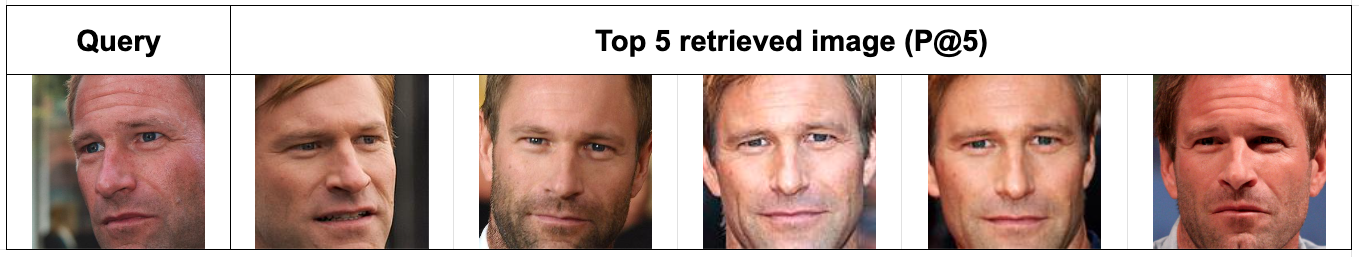
\includegraphics[width=0.8\textwidth]{images/face_retrieval_types.png} 
    \caption{Các dạng truy xuất ảnh mặt người}
    \label{fig:face_retrieval_types}
\end{figure}

\begin{figure}[htbp]
    \centering
    \includegraphics[width=0.6\textwidth]{images/similarity_retrieval_flow.png}
    \caption{Quy trình truy xuất theo độ tương đồng (tập trung của khóa luận)}
    \label{fig:similarity_flow}
\end{figure}

Khóa luận tập trung vào \textbf{dạng thứ hai – truy xuất theo độ tương đồng}, với đầu vào là ảnh khuôn mặt truy vấn và đầu ra là \( K \) ảnh có độ tương đồng đặc trưng cao nhất, không ràng buộc danh tính. Các dạng còn lại được đề cập để làm rõ bối cảnh bài toán.

\section{Thách thức bài toán}
Việc xây dựng một mô hình truy xuất ảnh mặt người vừa gọn nhẹ vừa có khả năng mở rộng trên tập dữ liệu quy mô lớn phải đối mặt với nhiều thách thức đáng kể. Các thách thức này có thể được phân loại thành ba nhóm chính: thách thức liên quan đến dữ liệu, kiến trúc mô hình xác hiệu suất hệ thống. 

Thứ nhất, về mặt dữ liệu, các hệ thống phải xử lý sự biến đổi phức tạp vốn có trong ảnh mặt người. Một mặt, sự biến đổi trong cùng một danh tính (biến đổi nội lớp) là rất lớn, khi hình ảnh của cùng một các nhân có thể khác biệt đáng kể do sự thay đổi về góc chụp, điều kiện ánh sáng, biểu cảm, quá trình lão hoá, hay sự che khuất bởi các vật thể như khẩu trang, kính râm. Mặt khác, độ tương đồng giữa các biến đổi nội lớp lại có thể rất thấp, khi những cá nhân khác biệt lại sở hữu các đặc điểm khuôn mặt tương tự. Tình trạng này đòi hỏi mô hình phải có khả năng học được một không gian đặc trưng vừa đủ mạnh mẽ để khái quát hoá các biến thể trong cùng một lớp, vừa đủ sức phân biệt để tách bạch các lớp khác nhau. Thêm vào đó, quy mô dữ liệu khổng lồ với hàng triệu đến hàng tỷ hình ảnh làm gia tăng cấp số nhân chi phí tính toán và lưu trữ, đặt ra yêu cầu cấp thiết về hiệu quả trong cả quá trình huấn luyện và truy xuất.

Thứ hai, về kiến trúc mô hình, thách thức cốt lõi nằm ở sự đánh đổi giữa độ chính xác và hiệu quả tính toán. Các mô hình học sâu hiện đại có dung lượng lớn thường đạt độ chính xác cao nhờ khả năng biểu diễn mạnh mẽ, nhưng lại đòi hỏi tài nguyên tính toán khổng lồ, không phù hợp cho việc triển khai trên các thiết bị tài nguyên hạn chế. Do đó, việc thiết kế một kiến trúc mạng gọn nhẹ nhưng vẫn duy trì được khả năng trích xuất đặc trưng có sức phân biệt cao là một bài toán khó. Điều này gắn liền với thách thức về việc học một biểu diễn đặc trưng cô đặc. Việc giảm số chiều của vector đặc trưng là tối quan trọng để tiết kiệm bộ nhớ và tăng tốc độ tìm kiếm, nhưng quá trình này có nguy cơ làm mất mát thông tin nhận dạng quan trọng.

Cuối cùng, về hiệu suất hệ thống, mô hình phải đáp ứng được yêu cầu về tốc độ truy xuất trong thời gian thực. Với có sở dữ liệu quy mô lớn, việc tìm kiếm tuần tự qua toàn bộ dữ liệu là bất khả thi về mặt thời gian. Điều này đòi hỏi phải tích hợp các thuật toán lập chỉ mục và tìm kiếm lân cận gần đúng hiệu quả. Hơn nữa, mục tiêu cuối cùng là triển khai trên các thiết bị biên như điện thoại di động hay camera thông minh, vốn bị giới hạn nghiêm ngặt về năng lực xử lý, bộ nhớ và năng lượng. Do đó, toàn bộ hệ thống, từ mô hình trích xuất đặc trưng đến thuật toán tìm kiếm, phải được tối ưu hoá để hoạt động hiệu quả trong một môi trường tài nguyện bị ràng buột chặt chẽ.

\section{Giới hạn bài toán}
Mặc dù bài toán truy xuất ảnh mặt khuôn mặt người mang tính ứng dụng cao và rộng rãi trong nhiều lĩnh vực, khoá luận này chỉ tập trung vào một số khía cạnh cụ thể nhằm đảm bảo tính khả thi, tập trung sâu và phù hợp với nguồn lực nghiên cứu hạn chế của một công trình tốt nghiệp. Các giới hạn được xác định rõ ràng để tránh mở rộng phạm vi quá mức, đồng thời duy trình tính khả thi trong việc thực nghiệm và đánh giá.

Đầu tiên, nghiên cứu chỉ xem xét dạng truy xuất dựa trên độ tương đồng, tức là tìm kiếm các ảnh có đặc trưng khuôn mặt gần giống nhất với ảnh truy vấn mà không ràng buộc về mặc danh tính hoặc các thuộc tính phụ trợ. Việc loại trừ các dạng truy xuất theo danh tính và theo đặc trưng giúp tập trung nguồn lực vào việc tối ưu hoá không gian đặc trưng và thuật toán tìm kiếm gần đúng, tránh phức tạp hoá bởi các yêu cầu bổ sung như phân loại thuộc tính hoặc kiểm tra danh tính chính xác. Điều này phù hợp với mục tiêu chính là xây dựng mô hình gọn nhẹ, nhưng đồng thời hạn chế khả năng áp dụng trực tiếp vào các hệ thống yêu cầu truy xuất đa dạng hơn, chẳng hạn như nhận dạng người hoặc lọc ảnh theo thuộc tính cụ thể. 

Thứ hai, mặc dù mô hình được thiết kế và tối ưu hoá chủ yếu dành cho các thiết bị có tài nguyên hạn chế, chẳng hạn như thiết bị di động hoặc thiét bị biên, với các ràng buộc nghiêm ngặt về công suất tính toán, bộ nhớ và năng lượng, khoá luận vẫn sử dụng nền tảng đám mây Kaggle với GPU T4x2 để thực hiện huấn luyện và đánh giá ban đầu do hạn chế về tài nguyên phần cứng thực tế. Các chỉ số hiệu suất như độ chính xác trung bình trung vị (MAP), độ chính xác hàng đầu (Top-K) và thời gian truy vấn mỗi mili giây được đo lường trên môi trường này, với thời gian truy vấn dựa trên xử lý theo lô cho toàn bộ tập kiểm tra và các lần tìm kiếm gần đúng, dẫn đến ước lượng có thể không phản ánh chính xác thời gian truy vấn đơn lẻ hoặc chi phí phụ trợ trong môi trường thực tế. Do đó, nghiên cứu không khám phá việc triển khai hoặc đánh giá trên thiết bị biên cụ thể, chấp nhận rằng các kết quả đo lường dựa trên hần cứng cao cấp có thể không đại diện đầy đủ cho hiệu suất trên thiết bị hạn chế và bỏ qua các yếu tốt như khả năng mở rộng quy mô ngang trong môi trường đám mây đầy đủ, tích hợp với các dịch vụ như Google Cloud Vision hoặc AWS Rekonition, hoặc đo lường độ trễ thực tế dưới ràng buộc năng lượng.

Về mặt dữ liệu, khoá luận sử dụng các tập dữ liệu tiêu chuẩn trong lĩnh vực nhận diện khuôn mặt, chẳng hạn như VGGFace2 hoặc các tập dữ liệu tương tự với quy mô hàng triệu ảnh, để huấn luyện và đánh giá mô hình. Tuy nhiên, nghiên cứu không mở rộng đến các tập dữ liệu thực tế có quy mô hàng tỷ ảnh hoặc dữ liệu thời gian gần thực từ các hệ thống giám sát lớn, do hạn chế về tài nguyên tính toán và thời gian thực hiện. Điều này có nghĩa là mô hình có thể chưa được kiểm chứng đầy đủ trong các điều kiện dữ liệu thực tế đa dạng hơn về biến đổi môi trường, chẳng hạn như ảnh có độ phân giải thấp, che khuất nghiêm trọng, hoặc biến đổi do điều kiện thời tiết khắc nghiệt. Ngoài ra, tập dữ liệu chủ yếu đựa trên các nguồn công khai phương Tây, có thể dẫn đến thiên kiến văn hoá chúng tộc, hạn chế khả năng tổng quát hoá cho các quần thể đa dạng hơn, như ở Việt Nam hoặc các quốc gia Châu Á.

Thứ ba, khoá luận không đề cập đến các vấn đề liên quan đến an ninh, bảo mật dữ liệu và quyên riêng tư. Cụ thể, không xem xét các quy định pháp lý như Quy định bảo vệ dữ liệu chung (GDPR) của Liên minh Châu Âu, hoặc các biện pháp bảo vệ dữ liệu cá nhân trong quá trình lưu trữ và xử lý ảnh khuôn mặt. Đồng thời, nghiên cứu bỏ qua các dạng tấn công đối kháng, chẳng hạn như việc tạo ra các ảnh đầu vào bị thay đổi tinh vi nhằm làm suy giảm hiệu suất mô hình, vốn là một thách thức lớn trong các ứng dụng thực tế như an ninh công cộng. Việc không tích hợp các kỹ thuật phòng thủ có thể làm giảm tính mạnh mẽ của mô hình trong môi trường thù địch.

Về phương diện kỹ thuật, các cải tiến chỉ tập trung vào kiến trúc mô hình và quá trình lượng tử hoá, mà không bao gồm các kỹ thuật hậu xử lý nâng cao như sắp xếp lại kết quả (re-ranking) dựa trên đặc trưng địa phương hoặc kết hợp đa phương thức, ví dụ như tích hợp với dữ liệu văn bản hoặc âm thanh để tăng cường độ chính xác. Điều này giúp giữ mô hình đơn giản và gọn nhẹ, nhưng đồng thời hạn chế tiềm năng cải thiện hiệu suất trong các kịch bản phức tạp hơn.

Cuối cùng, khoá luận không xem xét các yếu tố thực tế như biến động mạng lưới, tích hợp hệ thống toàn diện với các thành phần phần mềm khác, hoặc đánh giá trên đa nền tnagr phần cứng. Do đó, kết quả có thể chưa phản ảnh đầy đủ hiệu suất trong môi trường triển khai thực tế, nơi các yếu tố bên ngoài như tải hệ thống hoặc biến đổi phần cứng có thể ảnh hưởng đáng kể. Tổng thể, các giới hạn này được đặt ra để đảm bảo nghiên cứu tập trung vào mục tiêu cốt lõi là phát triển một kiến trúc gọn nhẹ cho truy xuất ảnh khuôn mặt trên dữ liệu lớn, đồng thời mở ra các hướng mở rộng trong các công trình nghiên cứu tương lai.

\section{Hướng tiếp cận}
Để giải quyết bài toán truy xuất ảnh khuôn mặt trên tập dữ liệu lớn với yêu cầu về kiến trúc gọn nhẹ và tốc độ cao, khoá luận đề xuất một hướng tiếp cận cải tiến dựa trên phương pháp Mạng lượng tử hoá tích chập trực chuẩn (OPQN) \cite{opqn}. Cụ thể, chúng tôi thay thế mạng xương sống ResNet20 trong OPQN gốc bằng EdgeFace - một kiến trúc lai giữa Mạng nơ-ron tích chập (CNN) và biến đổi (Transformer), được thiết kế đặc biệt cho nhận diện khuôn mặt trên thiết bị biên.

\subsection{Trích xuất đặc trưng sử dụng EdgeFace}
Ở giai đoạn đầu, ảnh khuôn mặt sau tiền xử lý (chuẩn hoá kích thước, căn chỉnh) được đưa vào EdgeFace thay cho ResNet20 nhưu trong OPQN gốc. EdgeFace là một mô hình nhẹ, với các biến thể EdgeFace-XS hoặc EdgeFace-XXS chỉ có khoảng 1-2 triệu tham số và ~150 MFLOPs (trên ảnh 112x112) thấp hơn nhiều so với hơn 300 MFLOPs của ResNet20. Điều này giúp giảm gánh nặng tính toán, đặc biệt khi triển khai trên thiết bị di động. 

Kiến trúc EdgeFace kết hợp các khối CNN với các module Transformer tối ưu hóa, bao gồm Hợp tuyến tính hạng thấp (Low-Rank Linear - LoRaLin) để giảm số tham số và Chú ý chuyển vị độ sâu tách biệt (Split Depth-wise Transpose Attention - STDA) để xử lý hiệu quả đặc trưng cục bộ và toàn cục. Kết quả là một vector đặc trưng chiều $ d = 512 $, được chuẩn hóa lên siêu cầu đơn vị (unit hypersphere) để đảm bảo tính ổn định và so sánh nhất quán trong không gian đặc trưng.

\subsection{Lượng tử hóa và mã hóa đặc trưng}
Sau bước trích xuất, vector đặc trưng được đưa vào cơ chế lượng tử hoá tích chập trực chuẩn của OPQN. Quá trình này chia vector thành các không gian con và mã hoá bằng các bộ mã, dựa trên cơ sở trực chuẩn biến đổi cosine rời rạc II (DCT-II), giúp giảm lỗi lượng tử hoá. 

Quá trình này chia vector $f \in R^d$ thành $m$ không gian con $f_i$, mỗi phần từ được mã hoá bằng các bộ mã $C_i = {c_{i1},..c_{ik}}$, trong đó $k = 2^b$ với $b$ là số 

\section{Đóng góp}
\section{Tổ chức khóa luận}
\section{Tổng kết}

\newpage


%Tóm tắt luận văn được trình bày nhiều nhất trong 24 trang in trên hai mặt giấy, cỡ chữ Times New Roman 11 của hệ soạn thảo Winword hoặc phần mềm soạn thảo Latex đối với các chuyên ngành thuộc ngành Toán.

%Mật độ chữ bình thường, không được nén hoặc kéo dãn khoảng cách giữa các chữ.
%Chế độ dãn dòng là Exactly 17pt.
%Lề trên, lề dưới, lề trái, lề phải đều là 1.5 cm.
%Các bảng biểu trình bày theo chiều ngang khổ giấy thì đầu bảng là lề trái của trang.
%Tóm tắt luận án phải phản ảnh trung thực kết cấu, bố cục và nội dung của luận án, phải ghi đầy đủ toàn văn kết luận của luận án.
%Mẫu trình bày trang bìa của tóm tắt luận văn (phụ lục 1).